\documentclass[12pt,titlepage]{article}
\usepackage{mathpazo}
\usepackage{color}
\usepackage[a4paper,lmargin={4cm},rmargin={2cm},tmargin={2.5cm},bmargin={2.5cm}]{geometry}
\usepackage[T1]{fontenc}
\usepackage[absolute,overlay]{textpos}
\usepackage[utf8]{inputenc}
\usepackage[ngerman]{babel}
\usepackage{blindtext}
\usepackage{graphicx}
\usepackage{wrapfig}
\usepackage{subfig}
\usepackage{multirow}
\usepackage{amsmath}
\usepackage{thmtools} 
\usepackage{amssymb} 
\usepackage{listings} 
\usepackage{siunitx}
\usepackage{tabularx}
\usepackage[pdfborder={0 0 0}]{hyperref}
\usepackage{breakurl}
\usepackage[onehalfspacing]{setspace}
\usepackage{cleveref}
\usepackage{smartdiagram}
\usepackage{placeins}
\lstset{numbers=left, numberstyle=\tiny, numbersep=5pt}
\lstset{language=Perl}

\begin{document}

\begin{titlepage}
\title{Deep-Q-Learning}
\date{27.02.2022}
\author{Janot George, Maurice Borries}
\maketitle
\end{titlepage}

\tableofcontents



\newpage
\section{Declaration of Authorship}
We hereby confirm that we have authored this Seminar paper independently and without use of others than the indicated sources. All passages (and codes) which are literally or in general matter taken out of publications or other sources are marked as such.
\\\\
Berlin, 27.02.2022, Janot George, Maurice Borries

\section{Einleitung}
Die technische Entwicklung hat sich in den letzten Jahrzehnten stark verändert, immer mehr Arbeitsprozesse werden automatisiert und von Maschinen übernommen. Dies wird in Zukunft eine noch größere Rolle spielen. Vor allem in dem Bereich des maschinellen Lernens. Aus diesem Grund haben wir uns mit der Thematik Q-Learning (QL) und Deep-Q-Learning (DQL) befasst, da sie einen großen Teil des maschinellen Lernens ausmachen. Hierzu haben wir zwei Programme entwickelt, die das selbstständige Lernen einer Künstlichen Intelligenz (KI) veranschaulichen soll. Der agierende Teil der KI wird im weiteren als Agent bezeichnet. Um Q-Learning genauer zu erklären, haben wir eine KI entwickelt, die versuchen soll, aus einem Labyrinth zu gelangen und dazu auf das gelernte Wissen von den vorherigen Durchgängen zurückgreifen soll, um so einen Weg zu finden, schnellstmöglich aus dem Labyrinth zu gelangen. Für Deep-Q-Learning haben wir das bekannte Spiel Snake programmiert und den Agenten dieses spielen lassen. Bei dem Spiel ist es das Ziel, möglichst viele Äpfel zu essen, ohne dabei gegen die Wand zu stoßen oder sich selbst „zu essen“. Bevor wir allerdings explizierter auf die Beispiele eingehen können, erklären wir zunächst das grundlegende Konstrukt hinter dem maschinellen Lernen.

\section{Arten des maschinellen Lernens}
Als erstes muss man zwischen den drei Hauptmethoden des maschinellen Lernens unterscheiden: Dem Supervised Learning, dem Unsupervised Learning und dem Reinforcement Learning. Alle drei Methoden haben das Ziel einer KI eine bestimmte Aufgabe beizubringen und greifen dafür auf unterschiedliche Methodiken zurück.
Beim Supervised Learning ist das Ziel, der Künstlichen Intelligenz beizubringen, Vorhersagen treffen zu können. Das heißt, die KI soll mit der Zeit z. B. selbstständig Bilder unterscheiden können, hierzu wird dem Algorithmus ein beschrifteter Datensatz zur Verfügung gestellt, d. h. die KI erhält ein Bild mit der Beschriftung Apfel. Dadurch kann die KI selbstständig Bilder mit der Zeit unterscheiden und weiß gleichzeitig, ob das Bild ein Apfel ist oder nicht.
Der Unterschied zum Unsupervised Learning ist, dass der KI ein unbeschrifteter Datensatz zur Verfügung gestellt wird, d. h. sie versucht selbstständig Muster zu erkennen, indem sie zwischen z. B. der Form oder der Farbe von Bildern differenziert. Dies ermöglicht es der KI, Muster in den Bildern zu erkennen und diese nach Früchten zu sortieren.
Im weiteren Verlauf fokussiert sich diese Arbeit mehr auf eine Methode des Reinforcement Learnings. Beim Reinforcement Learning erhält die Künstliche Intelligenz keinen Datensatz. Sie lernt aus ihren eigenen Aktionen und Fehlern, speichert diese ab und versucht aus den gelernten Daten eine Strategie zu entwickeln.
Das Q-Learning ist ein Teilgebiet des Reinforcement Learnings. Die Daten werden durch sehr häufige und ausführliche Trial-and-Error-Abläufe gesammelt. Dies bedeutet, dass man den Agenten so lange Trainingsdurchläufe durchführen lässt, bis die gewünschte Lösung gefunden wird. Die KI erhält also im Vorfeld keinerlei Briefing und weiß somit nicht, welches Verfahren zum gewünschten Ergebnis führen wird. Sie kennt zudem auch das gewünschte Ziel nicht. Um dieses erreichen zu können, arbeitet das Reinforcement Learning mit einem Belohnungssystem, welches auf dem Zuckerbrot- und Peitschen-Prinzip basiert. Die KI muss also die Umgebung selbstständig erkunden und erhält für jede Aktion entweder Punkte oder ihr werden Punkte abgezogen. Man spricht hier von Belohnungen, als ein direktes Feedback, welches der KI mitgeteilt wird. Durch das Belohnungssystem versucht die KI die erhaltene Belohnung zu maximieren, indem sie eine Strategie entwickelt.
\\
\begin{table}
[ht] \caption{Arten d. Maschinellen Lernens} \label{tab:ArtdML}
\begin{tabular}{p{4,7cm}|p{4,7cm}|p{4,7cm}}
Supervised & Unsupervised & Reinforcement \\
\hline
&&\\
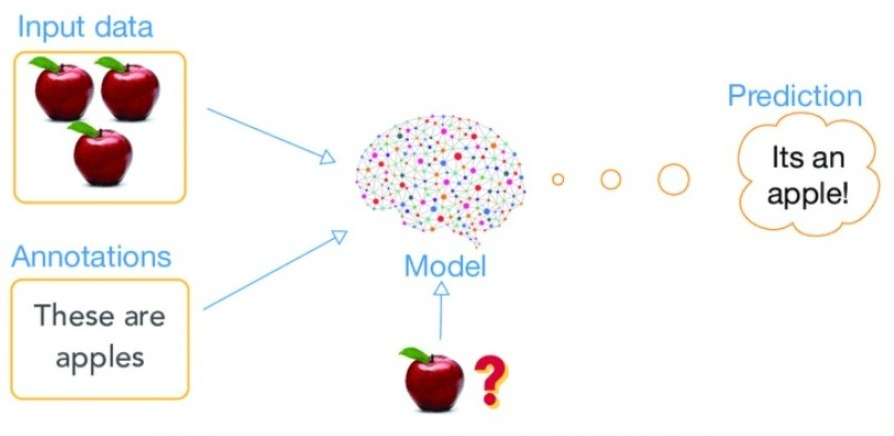
\includegraphics[width=4.7cm]{sup.png} & 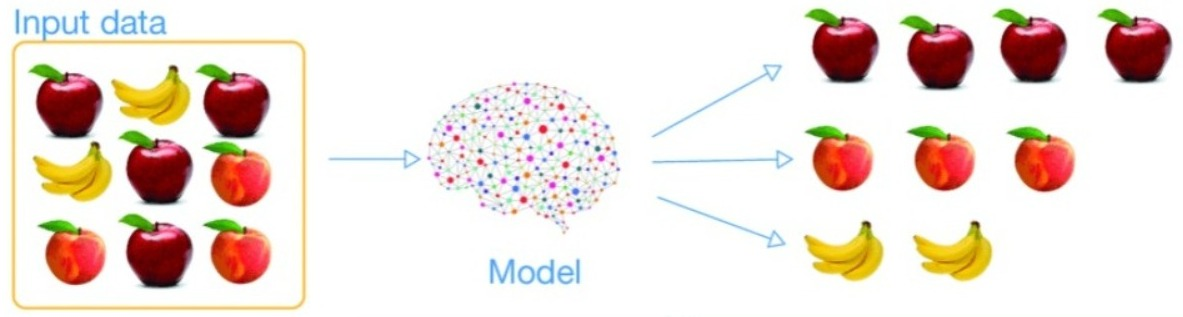
\includegraphics[width=4.7cm]{unsuper.png}  & 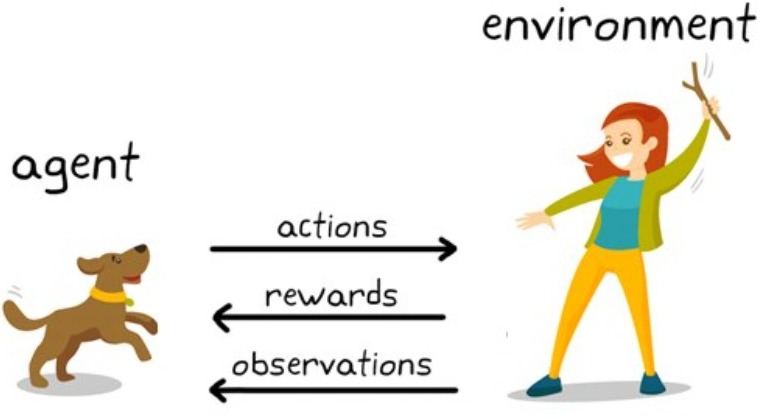
\includegraphics[width=4.6cm]{re.png} \\
fig:1 & fig:2 & fig:3\\
\hline
Vorhersagen treffen & Muster entdecken & Aus Fehlern selbstständig lernen
\end{tabular}
\end{table}

\section{Markov-Entscheidungsprozess}
Als Grundbaustein für den gesamten Algorithmus wird hierbei der Markov-Entscheidungsprozess herangezogen. Dieser ermöglicht es dem Agenten mit seiner Umgebung zu interagieren. Der Agent erhält für alle getätigten Aktionen in jedem Zustand, in dem er sich befindet, eine Belohnung. Ist dieser Wert negativ, kann man von Bestrafung reden. Definiert werden Aktion, Zustand und Belohnung wie folgt:
\begin{itemize}
\item Zustand der Umgebung zum Zeitpunkt $t$: $s_t$
\item Aktion der KI (des Agenten) zum Zeitpunkt $t$: $a_t$ 
\item Belohnung der Aktion $a_t$: $r_{t+1}$ 
\end{itemize}
Dabei ist die Dimension der Zeit eine Teilmenge der natürlichen Zahlen. Zudem gilt, dass immer nur ein Zustand der Umgebung zu jedem Zeitpunkt existiert und der Agent kann immer nur eine Aktion pro Zeitpunkt ausführen. 
\\\\
\begin{tabular}{c|p{1cm}|p{1cm}}
&&\\
\hline
& 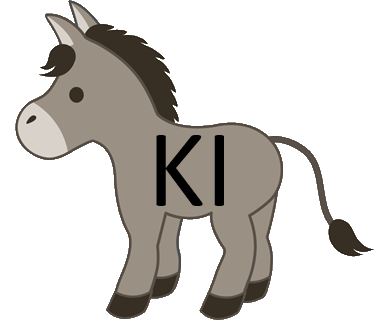
\includegraphics[width=1cm]{AI.png} & 
\includegraphics[width=0.5cm]{Target.png}\\
\hline
&&
\end{tabular}
$s_t$ \begin{tabular}{c|p{1cm}|p{1cm}}
&&\\
\hline
& 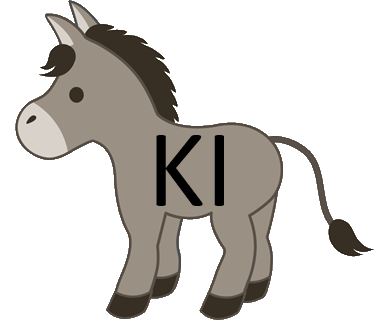
\includegraphics[width=1cm]{AI.png} & 
\includegraphics[width=0.5cm]{Target.png}\\
\hline
&&
\end{tabular}
$a_t$ \begin{tabular}{c|p{1cm}|p{1cm}}
&&\\
\hline
&& 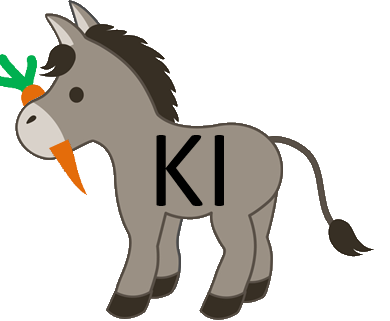
\includegraphics[width=1cm]{Reward.png}\\
\hline
&&
\end{tabular}
$r_{t+1}$\\\\
\begin{tabular}{c|p{1cm}|p{1cm}}
&&\\
\hline
&& 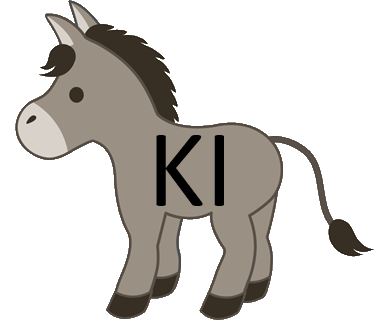
\includegraphics[width=1cm]{AI.png}\\
\hline
&&
\end{tabular}
$s_{t+1}$
\\\\
Es entsteht eine Schleife von Ereignissen, beginnend mit der Aktion in dem vorliegenden Zustand der Umgebung, gefolgt von der Belohnung und der Änderung des Zustandes.
\\\\
In den beiden Programmen haben die Komponenten folgende Struktur:
\\
\begin{table}
[ht] \caption{Komponenten im QL und DQL} \label{tab:KQL}
\begin{tabular}{|l|l|p{2,5cm}|l|p{3,5cm}|}
\hline
& Agent & Zustand & Umgebung & Aktion 
\\ \hline
QL & Esel im Labyrinth & Position im Labyrinth & Labyrinth & Bewegung in eine Richtung 
\\ \hline
DQL & Kopf der Schlange & Abstand des Kopfes zu Hindernissen und zum Apfel & Spielfeld & Bewegung in eine Richtung \\ \hline
\end{tabular}
\end{table}

\begin{textblock*}{2cm}(8.5cm,13.8cm)
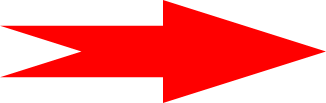
\includegraphics[width=1cm]{Action.png}
\end{textblock*}
\section{Exploration und Exploitation}
Da der Agent ohne Daten startet, auf die er zugreifen oder die er verarbeiten könnte, kann dieser keine gezielten Aktionen durchführen. Es bleibt ihm also nichts anderes übrig, als eine zufällige Aktion zu wählen. Diese Aktion wird als Exploration-Aktion bezeichnet. Der Agent erkundet hierbei das Umfeld und sammelt Daten, die er verarbeitet und in seinem Gedächtnis speichert. Da diese Aktionen keinerlei Strategien oder Ziele verfolgen, sind die Daten dieser Aktionen noch nicht sehr aussagekräftig, aber durch die Grundlage der Informationen, die sie liefern, kann der Agent nach und nach eine Strategie entwickeln. Wenn der Agent sich seinem Gedächtnis bedient und mit den gesammelten Informationen eine Aktion wählt, beschreibt man dies als Exploitation-Aktion. Der Agent nutz aus, was er gelernt hat und versucht seine Strategie auszuführen. Er erhält nun durch solche Aktionen wertvollere Daten, mit denen er seine Strategie ändert oder optimiert.
Die Erkundungsrate gibt an, wie hoch die Wahrscheinlichkeit ist, dass der Agent in einer Episode, eine Exploration-Aktion der Exploitation-Aktion vorzieht. Sie wird mit fortlaufenden Episoden jedoch reduziert, damit der Agent nun vermehrt auf seine Erfahrung zurückgreifen kann. Dies hat den Vorteil, dass der Agent am Anfang bzw. in den ersten Episoden hauptsächlich erkundet, um mit den Informationen ein generelles Verständnis seiner Umgebung und des Problems zu entwickeln. Er greift dann nach und nach immer öfter auf seine Erfahrungen zurück und optimiert auf diese Weise die Handhabung des Problems. Die neuen Informationen, die der Agent so sammelt, werden mit bereits bestehenden Erinnerungen verrechnet und anschließend im Gedächtnis aktualisiert. Dies ist das bevorzugte Vorgehen, um den Agenten ausgewogen zu trainieren.
\\\\
Die neue Erkundungsrate $\epsilon$ wird auf folgende Weise kalkuliert:
\begin{itemize}
\item $\epsilon = \epsilon_{min} + \frac{\epsilon_{max} - \epsilon_{min}}{e^{\epsilon_{red} \cdot Episodennummer}}$
\item $\epsilon_{max}$ : Erkundungsrate zu Beginn
\item $\epsilon_{red}$ : Reduktionswert der Erkundungsrate
\item $\epsilon_{min}$ : Minimale Erkundungsrate
\item Episodennummer ist die Anzahl der Episoden, die bereits durchgelaufen sind
\end{itemize}
Wobei dies Hyperparameter sind und vorab definiert und getestet werden müssen. 
In den Beispielen werden eine zufällige Zahl zwischen 1 und 0 generiert und abgeglichen, ob diese kleiner ist als die Erkundungsrate. Ist dies der Fall, wird eine zufällige Aktion ausgeführt, dies nennt man eine Exploration-Aktion. Ist dies nicht der Fall wird die bestmögliche Option aus der Q-Tabelle ausgeführt (Exploitation-Aktion).
Hinweis: Eine Abweichung von dieser Funktion oder Vorgehensweise kann unter Umständen und je nach Problem und Umfeld aber auch zielführend sein. Dies wird im weiteren Verlauf noch einmal verdeutlicht.

\section{Q-Learning-Episode}
Eine Episode ist als ein Problemlösungsversuch zu verstehen. Diese beginnt bei der erneuten Vorlegung des gleichen ungelösten Problems und endet beim Resultat des Agenten, welches durch viele Aktionen und Zustände beschrieben wird.
\\\\
\begin{center}
\smartdiagramset{text width=200, set color list={orange,red,pink}}
\smartdiagram[sequence diagram]{
{Startzustand},
{Q-Loop},
{Erkundung reduzieren}
}
\end{center}
Q-Loop:
\smartdiagramset{text width=130, set color list={red,red,red,red}}
\begin{center}
\smartdiagram[circular diagram:clockwise]{
{Exploration vs. Exploitation},
{Umgebung aktualisieren},
{Belohnung messen},
{Strategie aktualisieren}}
\end{center}
Im Startzustand wird die Episode initialisiert, der Zustand St=0 wird geschaffen. Dies bedeutet für die beiden Programme, dass der Esel im Labyrinth auf den Anfangspunkt gesetzt wird und für das Snake-Spiel wird ein Apfel generiert und die Schlange in Ausgangslänge und Position gebracht. Komponenten wie die Q-Tabelle oder momentaner Erkundungswert werden nicht zurückgesetzt.
Danach folgt ein Q-Loop. Dieser besteht hauptsächlich aus dem Markov-Entscheidungsprozess. Der Agent wählt zunächst eine Aktion basierend auf Exploration oder auf Exploitation aus und führt diese durch. Die Umgebung aktualisiert sich und der Agent erhält Informationen über den neuen Zustand sowie eine Belohnung. Anhand der Belohnung und des Zustandes kann nun mit der Annäherungsfunktion die Q-Tabelle aktualisiert werden. Dieser Loop wird so lange ausgeführt bis entweder die KI das Spiel durch einen Sieg oder eine Niederlage beendet oder das Spiel nach einer gewissen Schrittanzahl abgebrochen wird. 
Beim Ende der Episode wird nun die Erkundungsrate reduziert.

\section{Q-Funktionen}
Damit die KI die Qualität einer Aktion in einem Zustand bewerten kann, benötigt sie eine Funktion, um diese zu bemessen.
\\\\
Aktionsbewertungsfunktion: (Diskontierungsfaktor $\gamma$)
\begin{align*}
Q(s_t,a_t) = \mathbb{E} \left[ \sum\limits_{k=0}^{\infty} \gamma^{k} r_{t+k+1} \right]
\end{align*}
Die Aktionsbewertungsfunktion berechnet mithilfe der getätigten Aktion $a_t$ und dem Zustand $s_t$, in dem sie getroffen wurde, einen zu erwartenden Barwert aus allen zukünftigen Belohnungen, welche mit dem Diskontierungsfaktor $\gamma$ verrechnet werden. Problematisch hierbei ist, dass dies unendliche Rechenkapazität verlangt. Ein besserer Ansatz wäre es, dies iterativ zu berechnen. Die Bellman-Gleichung bietet die Lösung. 
\\\\
Bellman-Gleichung:
\begin{align*}
Q^{*}(s_t,a_t) = \mathbb{E} \left[ r_{t+1} + \gamma \max\limits_{a'} \left[ Q_T(s_{t+1}, a') \right] \right]
\end{align*}
Hier wird nur der Barwert der aktuellen und nächsten Belohnung berechnet. Wobei der nächste Wert jener ist, welcher bereits errechnet wurde und in der Q-Tabelle steht. Dieser ist erst nach vielen Iterationen präzise.
\\\\
LOSS-Funktion:
\begin{align*}
LOSS &= Q^{*}(s_t,a_t) - Q_T(s_t,a_t)
\end{align*}
Die LOSS-Funktion beschreibt die Differenz der Bellman-Gleichung und dem vorhandenen Wert in der Q-Tabelle bzw. später im DQL die Differenz der Bellman-Gleichung und dem Output des neuronalen Netzwerks. Das Ziel ist es, diesen Wert zu minimieren, um die Vorhersagen für den nächsten Schritt präziserer werden zu lassen.
Es wird eine Annäherungsfunktion aus der modifizierten LOSS-Funktion gebaut, um die Werte in der Tabelle zu aktualisieren. 
\\\\
Annäherungsfunktion:
\begin{align*}
Q_{T(neu)}(s_t,a_t) &= (1 - \alpha) \cdot Q_T(s_t,a_t) + \alpha \left[ r_{t+1} + \gamma \max\limits_{a'} \left[ Q_T(s_{t+1}, a') \right] \right]
\end{align*}
Hierfür wird ein weiterer Hyperparameter eingeführt. Die Lernrate $\alpha$ gibt an, wie die Gewichtung zwischen bereits bestehenden Informationen zu den erwarteten neuen Informationen liegt. Je höher die Lernrate ist, desto wertvoller sind die neuen Informationen. Liegt diese bei 1, werden die alten Erinnerungen bei der Aktualisierung nicht berücksichtigt. Liegt diese bei 0, wird die Tabelle nicht aktualisiert. Dieser Wert muss auch getestet werden, um das vorliegende Problem ideal lösen zu können. Ist die Lernrate zu niedrig, wird der Algorithmus in der Regel eine längere Zeit benötigen, um das Problem zu lösen. Ist sie jedoch zu hoch, werden ältere evtl. wichtige Informationen überschrieben und die entwickelte Strategie wird nie optimal werden.

\section{Q-Tabelle}
Die Q-Tabelle ist das Gedächtnis der Künstlichen Intelligenz beim Q-Learning. 
Sie hat eine Größe von Anzahl der Aktionen mal Anzahl der möglichen Zustände. So kann jede Aktion in jedem Zustand eine Bewertung erhalten.
Am Anfang ist die Q-Tabelle leer bzw. alle Einträge haben den Wert 0. 
Allerdings speichert die KI die Belohnungswerte, die sie nach einer Aktion erhält und überschreibt mit Hilfe der Annäherungsfunktion den alten Wert. Abhängig davon, ob die Entscheidung der KI gut oder schlecht war, fällt die Belohnung positiv oder negativ aus. Da die Werte nach jedem Durchgang überschrieben werden, wird die Aussagekraft der Tabelle präzisier. In dem Beispiel gibt es vier Aktionen, welche der Agent ausführen kann. Er kann einen Schritt nach oben, unten, rechts und links machen. Wenn der Schritt des Agenten ihn näher an das Ziel bringt, in dem Fall will der Esel die Möhre erreichen, fällt die Belohnung zu seinen Gunsten aus. Wenn die KI eine Exploitation-Aktion durchführt, wählt sie zuerst die Spalte in der 
Q-Tabelle aus, die ihrem Zustand entspricht. Danach wählt sie die Aktion aus, welche den höchsten Wert besitzt und führt diese aus. Dies nennt man „Greedier-Strategie“. Diese Strategie ist hierbei optimal, da es die Aufgabe des Agenten ist, schnellstmöglich aus dem Labyrinth zu gelangen.
\\\\
\begin{table}
[ht] \caption{Q-Tabelle Beispiel} \label{tab:QTB}
\begin{tabular}{|c|c|c|c|c|c|c|}
\hline
&&&&&&\\
& 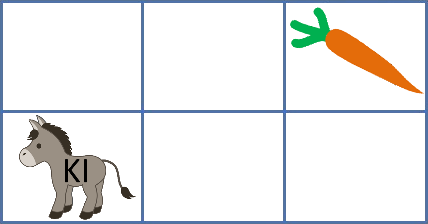
\includegraphics[width=1.8cm]{p1.png} & 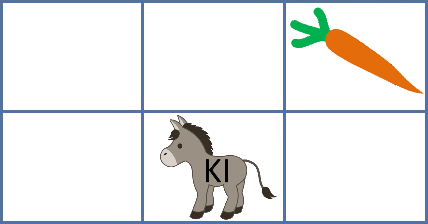
\includegraphics[width=1.8cm]{p2.png} & 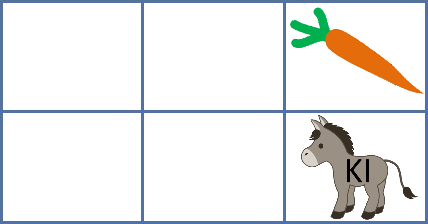
\includegraphics[width=1.8cm]{p3.png} & 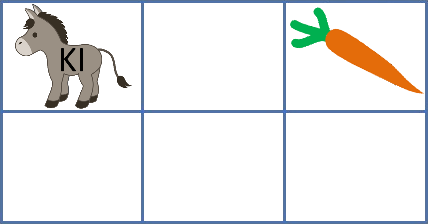
\includegraphics[width=1.8cm]{p4.png} & 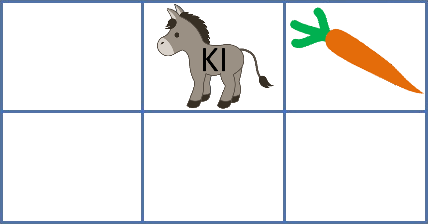
\includegraphics[width=1.8cm]{p5.png} & 
\includegraphics[width=1.8cm]{p6.png} \\
\hline
&&&&&&\\
{\huge $\Uparrow$} & 0,23 & 0,34 & 1 & -0,24 & -0,39 & 0\\
&&&&&&\\
\hline
&&&&&&\\
{\huge $\Downarrow$} & -0,52 & -0,49 & -0,32 & -0,05 & -0,03 & 0\\
&&&&&&\\
\hline
&&&&&&\\
{\huge $\Rightarrow$} & 0,24 & 0,45 & -0,38 & 0,55 & 1 & 0\\
&&&&&&\\
\hline
&&&&&&\\
{\huge $\Leftarrow$} & -0,59 & -0,15 & -0,15 & -0,34 & -0,03 & 0\\
&&&&&&\\
\hline
\end{tabular}
\end{table}

\section{QL-Beispiel}
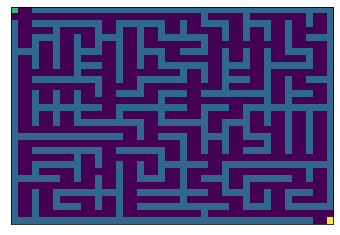
\includegraphics[width=12cm]{Laby.png}

plot:1\\\\
Um den Unterschied zwischen Exploration und Exploitation besser zu verstehen, wird dies mit dem Beispiel des Labyrinths veranschaulicht. Dazu werden die Erkundungsratenparameter geändert, während die anderen Parameter gleichbleiben.
Im folgenden Beispiel wird der Agent nur nach der Exploration-Strategie handeln, das heißt, die Exploration-Rate liegt bei 1 und wird nach jedem Durchgang nur minimal reduziert. Dies hat zur Folge, dass der Agent versucht, lediglich durch „raten“ den richtigen Weg aus dem Labyrinth zu finden und greift dabei nur sehr selten auf das Wissen der Q-Tabelle zurück.
\\\\
\begin{tabular}{c}
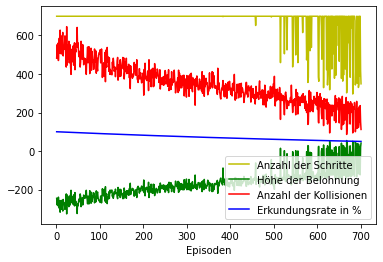
\includegraphics[width=12cm]{QL_Laby_1.png}
\end{tabular}

plot:2\\\\
Wie man sehr gut erkennen kann, ist die Anzahl der Kollisionen durchgehend sehr hoch und auch die Höhe der Belohnung ist sehr schwankend. Außerdem schafft der Agent es nur selten ins Ziel zu gelangen.
\\\\
\begin{tabular}{c}
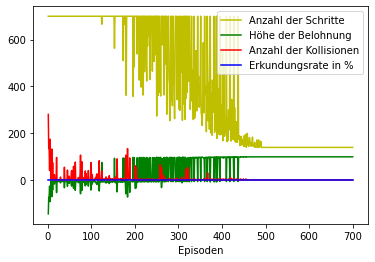
\includegraphics[width=12cm]{QL_Laby_2.png}
\end{tabular}

plot:3\\\\
Wenn man dies nun damit vergleicht, dass der Agent sich nur an die Exploitation-Strategie hält. Das bedeutet, er erkundet so gut wie gar nicht die Umgebung und greift lediglich auf die Informationen der Q-Tabelle zurück und entscheidet danach seine nächste Aktion. Da die Q-Tabelle am Anfang leer ist braucht die KI ein paar Episoden, um Informationen zu sammeln, auf die sie dann zurückgreifen kann. Man kann sehr gut erkennen, dass nach schon kurzer Zeit die Kollisionen sich minimieren und auch die Höhe der Belohnung ist konstant. Dies hat die Form eines „Brute-Force-Algorithmus“. Fehlerhafte Aktionen werden nie erneut versucht und die erste gefundene Strategie wird ausschließlich verfolgt.
\\\\
\begin{tabular}{c}
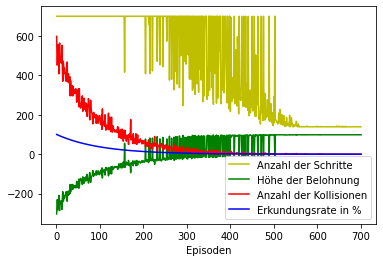
\includegraphics[width=12cm]{QL_Laby_3.png}
\end{tabular}

plot:4\\\\
Bei einer Kombination aus beiden Strategien, handelt der Agent am Anfang mehr nach der Exploration-Strategie und im Laufe der Zeit wird Erkundungsrate immer weiter reduziert und der Agent greift mehr auf das bereits gelernte Wissen zurück. Wie man hier gut erkennen kann, sieht die Entwicklung ähnlich aus, wie in dem Beispiel, bei dem der Agent nur auf das Wissen zurückgreift. Man könnte denken, dass nur auf das Wissen zurückgreifen, die beste Entscheidung ist. 
Das Problem hierbei ist allerdings, dass wenn der Agent einen Weg aus dem Labyrinth gefunden hat, er immer den gleichen Weg laufen wird, auch wenn dieser gar nicht der Schnellste ist. Bei einer Kombination aus beiden Strategien findet der Agent schnell den Weg ins Ziel und kann dabei auch noch Abkürzungen durch die Erkundung finden.

\section{Grenzen des Q-Learnings}
Je nachdem wie komplex die Problematik ist, werden die Grenzen des Q-Learnings schnell ersichtlich. Das Q-Learning ist für das Labyrinth Beispiel optimal, aber wenn der Zustand der Umgebung mehrere Features besitzt, desto größer muss die Q-Tabelle werden und umso mehr Rechenkapazität wird benötigt. Die benötigte Zeit zum Trainieren wird exponentiell wachsen, da alle Zustände erkundet und alle Aktionen mehrfach ausgeführt werden müssen.  Aus diesem Grund wird bei umfangreicheren Aufgabenstellungen auf das Deep-Q-Learning zurückgegriffen. Hierbei wird ein Ersatz für die Q-Tabelle benötigt. Dies gelingt durch den Einsatz eines neuronalen Netzwerks. Denn neuronale Netze sind in der Lage, große Mengen von unstrukturierten und komplexen Daten auszuwerten und sich zu optimieren. 
Sie bestehen aus mehreren Ebenen, die Input-Ebene, welche den Input aufnimmt, mehrere versteckte Ebenen, die die Berechnungen vornehmen und der Output-Ebene, in der die Ergebnisse bereitgestellt werden. Bei einem neuralen Netzwerk werden vor dem ersten Durchlauf die Gewichtungen zufällig gewählt, weshalb der Output zunächst ebenfalls zufällig ist. 
Zu Beginn ist das Netzwerk wie die Q-Tabelle aufgebaut, das heißt, beide können noch keinen zuverlässigen Output generieren.  Das Netzwerk muss auf eine andere Art trainiert werden, hierfür benötigt man einen Erinnerungsspeicher. Dieser hat eine festgelegte Größe für die Anzahl der Erinnerungen, die gespeichert werden sollen, damit hier ebenfalls die Datenmenge nicht überhandnimmt. Abgespeichert werden Erinnerungen wie folgt:
\begin{align*}
(s_t,a_t,r_{t+1},s_{t+1})
\end{align*}
Dieses enthalten folgende Informationen: Zustand zum Zeitpunkt t, ausgewählte Aktion zum Zeitpunkt t, erhaltene Belohnung als Resultat der Aktion und Zustand des nachfolgenden Zeitpunktes t+1.
\\\\
Es wird aus diesem Speicher eine Anzahl zufälliger Erinnerungen ausgewählt, welche als Input an das neuronale Netz gesendet werden. Dort wird dann die Gewichtung so angepasst, dass die LOSS-Funktion reduziert werden kann. Dies bewirkt, dass die Strategie des Netzwerkes verbessert wird. Die Auswahl der zufälligen Erinnerungen hat den Vorteil, dass keine Korrelationen bzw. kein Zusammenhang der einzelnen Erinnerungen besteht. Das Netzwerk wird auf diese Weise auf verschiedene Erinnerungen trainiert und nicht nur auf eine Kette von Aktionen. Dies bewirkt, dass die Strategie für verschiedene Situationen des Agenten verbessert wird. Wenn die Speicherkapazität erreicht ist, werden die ältesten Erinnerungen, welche qualitativ schlechter sind, gelöscht. Sie stammen aus einem veralteten Strategienetzwerk und sind aus diesem Grund nicht so aussagekräftig, wie die neu dazugewonnenen Erinnerungen und wurden deshalb vom Netzwerk im Vorfeld einkalkuliert und schließlich entfernt. 

\section{Deep-Q-Learning-Episode}
Der Ablauf einer Episode beim Deep-Q-Learning ist ähnlich wie der einer Q-Learning-Episode. 
\\\\
DQ-Loop:
\smartdiagramset{text width=130, set color list={red,red,red,red}}
\begin{center}
\smartdiagram[circular diagram:clockwise]{
{Exploration vs. Exploitation},
{Umgebung aktualisieren},
{Belohnung messen},
{Netzwerk trainieren}}
\end{center}
Der einzige Unterschied besteht darin, wie im DQ-Loop das Netzwerk trainiert wird. Das Training erfolgt mit derselben Häufigkeit wie beim Q-Learning. Die Entscheidung des Netzwerkes, welche Aktion gewählt wird, hat nur sehr geringen bis keinen Einfluss auf das Training, da hier mit zufälligen Erinnerungen gearbeitet wird. Das Netzwerk trifft im Q-Loop eine Entscheidung für die nächste Aktion, wenn eine Exploitation-Aktion gewählt wurde. Die Exploration-Aktion erfolgt genau wie beim Q-Learning.

\section{Aufbauänderungen beim Deep-Q-Learning}
Wird nur ein neuronales Netzwerk installiert, übernimmt dieses folgende Aufgaben: 
Wird eine Exploitation-Aktion gewählt, wird der Zustand als Input an das Netzwerk gegeben. Dieses liefert dann für jede mögliche Aktion einen Wert. Ähnlich wie in der Zustandsspalte der Q-Tabelle. Hier wird auch die „Greedier-Strategie“ angewendet und die Aktion mit dem höchsten Wert gewählt. Um den LOSS-Wert beim Training auszurechnen, wird das Ergebnis der Bellmann-Gleichnung benötigt sowie die Bewertung der Aktion:
\\\\
LOSS-Funktion:
\begin{align*}
LOSS &= \left[ r_{t+1} + \gamma \max\limits_{a'} \left[ Q(s_{t+1}, a') \right] \right] - Q(s_t,a_t)
\end{align*}
\\
Erinnerung:
\begin{align*}
(s_t,a_t,r_{t+1},s_{t+1})
\end{align*}
Um den LOSS-Wert mit der Erinnerung auszurechnen, werden noch folgende Komponenten benötigt:
\begin{align*}
\max\limits_{a'} \left[ Q(s_{t+1}, a') \right]\\
Q(s_t,a_t)
\end{align*}
Für $Q(s_t,a_t)$ wird der Zustand $s_t$ als Input an das Netzwerk gegeben und dann der Output gewählt, welcher der Aktion $a_t$ entspricht.\\ 
Für den anderen Teil $\max\limits_{a'} \left[ Q(s_{t+1}, a') \right]$ wird der Folgezustand $s_{t+1}$ als Input an das Netzwerk gegeben. Beim Output wird ebenfalls die „Greedier-Option“ gewählt.
Wenn nur ein Netzwerk installiert wird, das alle Aufgaben übernimmt, kann dies zu Problemen führen. Der LOSS-Wert wird aus sich gleichzeitig ändernden Bewertungen berechnet. Dies kann zu einer Überschätzung führen. 
Um dies zu vermeiden, wird ein weiteres Netzwerk eingeführt. Das Deep-Q-Learning wird auf das Double-Deep-Q-Learning (DDQL) nach Hasselt aus dem Jahr 2015 erweitert. Das erste Netzwerk erhält den Namen: Strategienetzwerk und das Neue den Namen: Target-Netzwerk. Das Target-Netzwerk ist eine Kopie des Strategienetzwerkes, das nach einem fixen Zeitraum durch eine neuere Kopie des Strategienetzwerkes ersetzt wird. Das Strategienetzwerk gibt beim Training folgende Berechnung an das Target-Netzwerk weiter: $\max\limits_{a'} \left[ Q(s_{t+1}, a') \right]$. Da dieser Teil von dem „Vergangenheits-Netzwerk“ berechnet wird und dieses Netzwerk feste Gewichtungen besitzt, kann eine Überschätzung verringert werden.
Hinweis: In der älteren Version des DDQL von Hasselt aus dem Jahr 2010 wird nach einem fixen Zeitraum immer erneut zufällig ausgewählt, welches Netzwerk das Primäre, also das Strategienetzwerk und welches das Target-Netzwerk ist. In dem Verzeichnis wird die Datei als altDoubleDQSnake.py bezeichnet und die neue Version als DoubleDQSnake.py.
\\\\
Um die Überschätzung noch weiter zu minimieren, wird die Methodik noch weiter angepasst. Das Netzwerksystem wird zu Clipped-Deep-Q-Learning erweitert. Hierbei berechnen beide Netzwerke: $\max\limits_{a'} \left[ Q(s_{t+1}, a') \right]$ und der geringere Wert wird verwendet. Dies führt zu einer Unterschätzung, anstelle einer Überschätzung, die im Allgemeinen als besser eingeschätzt wird.
\\
\begin{table}
[ht] \caption{Aufgaben der Netzwerke} \label{tab:ADN}
\begin{tabular}{p{2cm}|p{3.7cm}|p{3.8cm}|p{3.8cm}}
& Deep-Q-Learning (DQL) & Double Deep-Q-Learning (DDQL) & Clipped Deep-Q-Learning (CDQL)\\
\hline
Strategie-Netzwerk & \begin{tabular}[c]{@{}l@{}}Exploitation\\$Q(s_t,a_t)$\\$\max\limits_{a'} \left[ Q(s_{t+1}, a') \right]$\end{tabular} & \begin{tabular}[c]{@{}l@{}}Exploitation\\$Q(s_t,a_t)$\end{tabular}         & \begin{tabular}[c]{@{}l@{}}Exploitation\\$Q(s_t,a_t)$\\$\max\limits_{a'} \left[ Q(s_{t+1}, a') \right]$\end{tabular}  \\
\hline
&&&\\
Target-Netzwerk  & & $\max\limits_{a'} \left[ Q(s_{t+1}, a') \right]$ & $\max\limits_{a'} \left[ Q(s_{t+1}, a') \right]$ \\
\end{tabular}
\end{table}

\section{Deep-Q-Learning Beispiel}
Die oben genannten Methodiken wurden alle auf das Spiel Snake angewendet. Wie an den Plots zu erkennen ist, sind Probleme aufgetreten. Dies kann entweder im Zusammenhang mit falsch gewählten Parametern oder falsch gewählten Netzwerkstrukturen stehen. Nach zahlreichen Versuchen und Änderungen, sowohl der Parameter, wie auch einer Anpassung der Netzwerkstrukturen, wurde das gewünschte Ziel trotzdem nicht erreicht.  
\\\\
\begin{tabular}{cc}
(Single)-Deep-Q-Learning & Double-Deep-Q-Learning(alt)\\
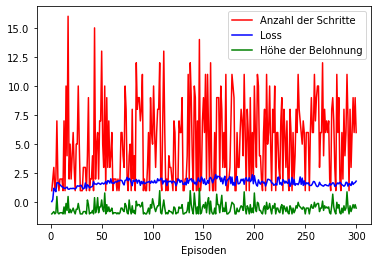
\includegraphics[width=7.2cm]{SDQL.png} & 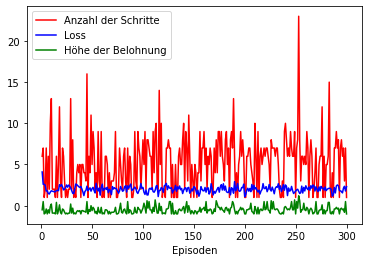
\includegraphics[width=7.2cm]{ADDQL.png}\\
&\\
Double-Deep-Q-Learning(neu) & Clipped-Deep-Q-Learning\\
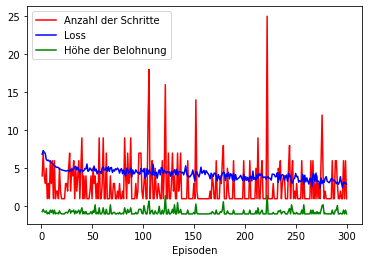
\includegraphics[width=7.2cm]{DDQL.png} & 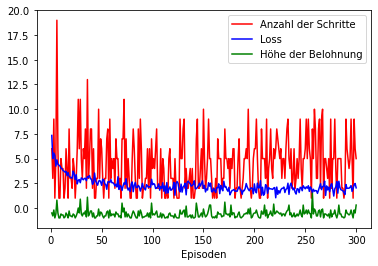
\includegraphics[width=7.2cm]{CDQL.png}
\end{tabular}

plot:5

\section{Fazit}
Wir sind zu dem Ergebnis gekommen, dass das maschinelle Lernen eine sehr interessante Art und Weise ist, mit neuen komplexen Problemen umzugehen. Dabei ist uns aufgefallen, dass schon kleine Aufgabenstellungen, die im ersten Moment nicht sehr komplex wirken, sehr zeitintensiv sind. Um für den Agenten eine geeignete Lösung für das Verlassen des Labyrinths zu finden, hat es zahlreiche Versuche benötigt, die optimalen Parameter festzulegen. Mit dem Deep-Q-Learning war dies sogar noch komplizierter und komplexer. Die Struktur des Netzwerkes ist für unser DQL-Beispiel nicht optimal und bietet demnach auch nicht so aussagekräftige Ergebnisse, wie bei unserem QL-Beispiel.
Wir sind der Auffassung, dass das maschinelle Lernen in Zukunft definitiv eine wesentliche Rolle in unserem Alltag spielen wird. Die Vorstellung, eine Maschine so trainieren zu können, dass sie z. B. den Aktienmarkt selbstständig analysiert und sichere Prognosen im Vorfeld erstellen kann, halten wir allerdings mit dem momentanen technischen Stand noch nicht für realisierbar. Wie wir in unserer Ausarbeitung bereits erwähnt haben, wird mit der steigenden Komplexität einer Problematik, eine sehr hohe Rechenleistung benötigt. Um am Aktienmarkt im Vorfeld Aussagen treffen zu können, werden sehr viele Datensätze benötigt, die momentan noch nicht so zur Verfügung stehen, um mit ihnen arbeiten zu können. Außerdem müsste man auch Faktoren berücksichtigen, wie z. B. Naturkatastrophen oder auch menschliches Versagen, die zu unvorhersehbaren Kursschwankungen führen können. 




\section{Abbildungsverzeichnis}
\begin{itemize}
\item[fig:1] supervised https://www.analyticsvidhya.com/blog/2019/04/introduction-deep-q-learning-python/ ; Zuletzt aufgerufen: 30.1.2022
\item[fig:2] unsupervised https://www.researchgate.net/figure/Supervised-learning-and-unsupervised-learning-Supervised-learning-uses-annotation$\_$fig1$\_$\\329533120 ; Zuletzt aufgerufen: 30.1.2022
\item[fig:3] reinforcement://www.kdnuggets.com/2019/10/mathworks-reinforcement-learning.html; Zuletzt aufgerufen: 30.1.2022
\item[Esel] https://de.cleanpng.com/png-b1ndvx/; Zuletzt aufgerufen: 22.11.2021
\item[plot:1] mit Python erstellt; Labyrinth, in dem sich der Esel bewegt
\item[plot:2] mit Python erstellt; Exploration-Durchlauf
\item[plot:3] mit Python erstellt; Exploitation-Durchlauf
\item[plot:4] mit Python erstellt; Exploration/Exploitation-Durchlauf
\item[plot:5] mit Python erstellt; Output der Snake Deep-Q-Learning Algorithmen
\end{itemize}

\section{Tabellenverzeichnis}
\listoftables

\section{Quellenverzeichnis}
\begin{itemize}
\item Richter, S. (2019) Statistisches und maschinelles Lernen, Berlin, Springer.
\item K.-L. Du and M. N. S. Swamy, Neural Networks and Statistical Learning.
\item Ilyas, Agakishiev: METIS: Reinforcement Learning, Humboldt-Universität zu Berlin, IRTG1792.HU-Berlin.de
\item https://www.learndatasci.com/tutorials/reinforcement-q-learning-scratch-python-openai-gym/ , Satwik Kansal, Brendan Martin, zuletzt abgerufen: 7.12.2021
\item https://ichi.pro/de/einfuhrung-in-das-reinforcement-learning-markov-\\entscheidungsprozess-7561377034876, ICHI.PRO, Laurenz Wuttke, zuletzt abgerufen: 7.12.2021
\item https://hci.iwr.uni-heidelberg.de/system/files/private/downloads/\\541645681/ dammann-reinfocement-learning-report.pdf ,Patrick Dammann, zuletzt abgerufen: 7.12.2021
\item http://www.informatik.uni-ulm.de/ni/Lehre/SS05/RL/vorlesung/rl03.pdf , F. Schwenker, zuletzt abgerufen: 7.12.2021
\item https://deeplizard.com/ , Chris and Mandy, zuletzt abgerufen: 7.12.2021
\item https://datasolut.com/neuronale-netzwerke-einfuehrung/ ,Laurenz Wuttke, zuletzt abgerufen: 7.12.2021
\item https://www.samyzaf.com/ML/rl/qmaze.html , zuletzt abgerufen: 7.12.2021
\item https://www-aitude-com.translate.goog/supervised-vs-unsupervised-vs-\\reinforcement/?$\_$x$\_$tr$\_$sl=en$\& \_$x$\_$tr$\_$tl=de$\& \_$x$\_$tr$\_$hl=de$\& \_$x$\_$tr$\_$pto\\=op, sc ; zuletzt abgerufen: 27.1.2022
\item https://www.trendreport.de/anwendung-des-machine-learning-bei-der-\\analyse-von-kapitalmaerkten/, Tobias Waning, Alexander Brun, Hendrik von der Haar, zuletzt abgerufen: 27.1.2022
\end{itemize}
\end{document}